コードの理解は、ソフトウェア開発において非常に重要です。
開発者の作業には、コードの作成だけでなく、他のチームメンバーによる修正のレビュー、プロジェクト全体の管理、潜在的に有用なライブラリの検証などが含まれます。
これらのタスクを正常に完了するには、正しいコードの理解が必要です。
しかし、コードの理解度は無視できないほどの時間と労力を必要とすることがあります。

実際には、開発者はプロジェクト全体ではなく、コードの一部、つまり\ textit {コードピース}をよく理解する必要があります。
たとえば、コードの一部(関数やクラスなど)のバグを修正するように求められます。
コードレビューは、コード部分の理解を必要とする別のアクティビティです。
所与のコード片(例えば、リビジョンおよびレビューのログ)に関連する情報は、その開発コンテキストを提供することによってコード理解を容易にすることができる。
これらの明白なニーズにもかかわらず、既存のシステムおよびツールは、開発者がコード片のためにそのような情報をうまく入手するのを助けるものではない。

% \begin{figure}[!b]
%   \centering
%   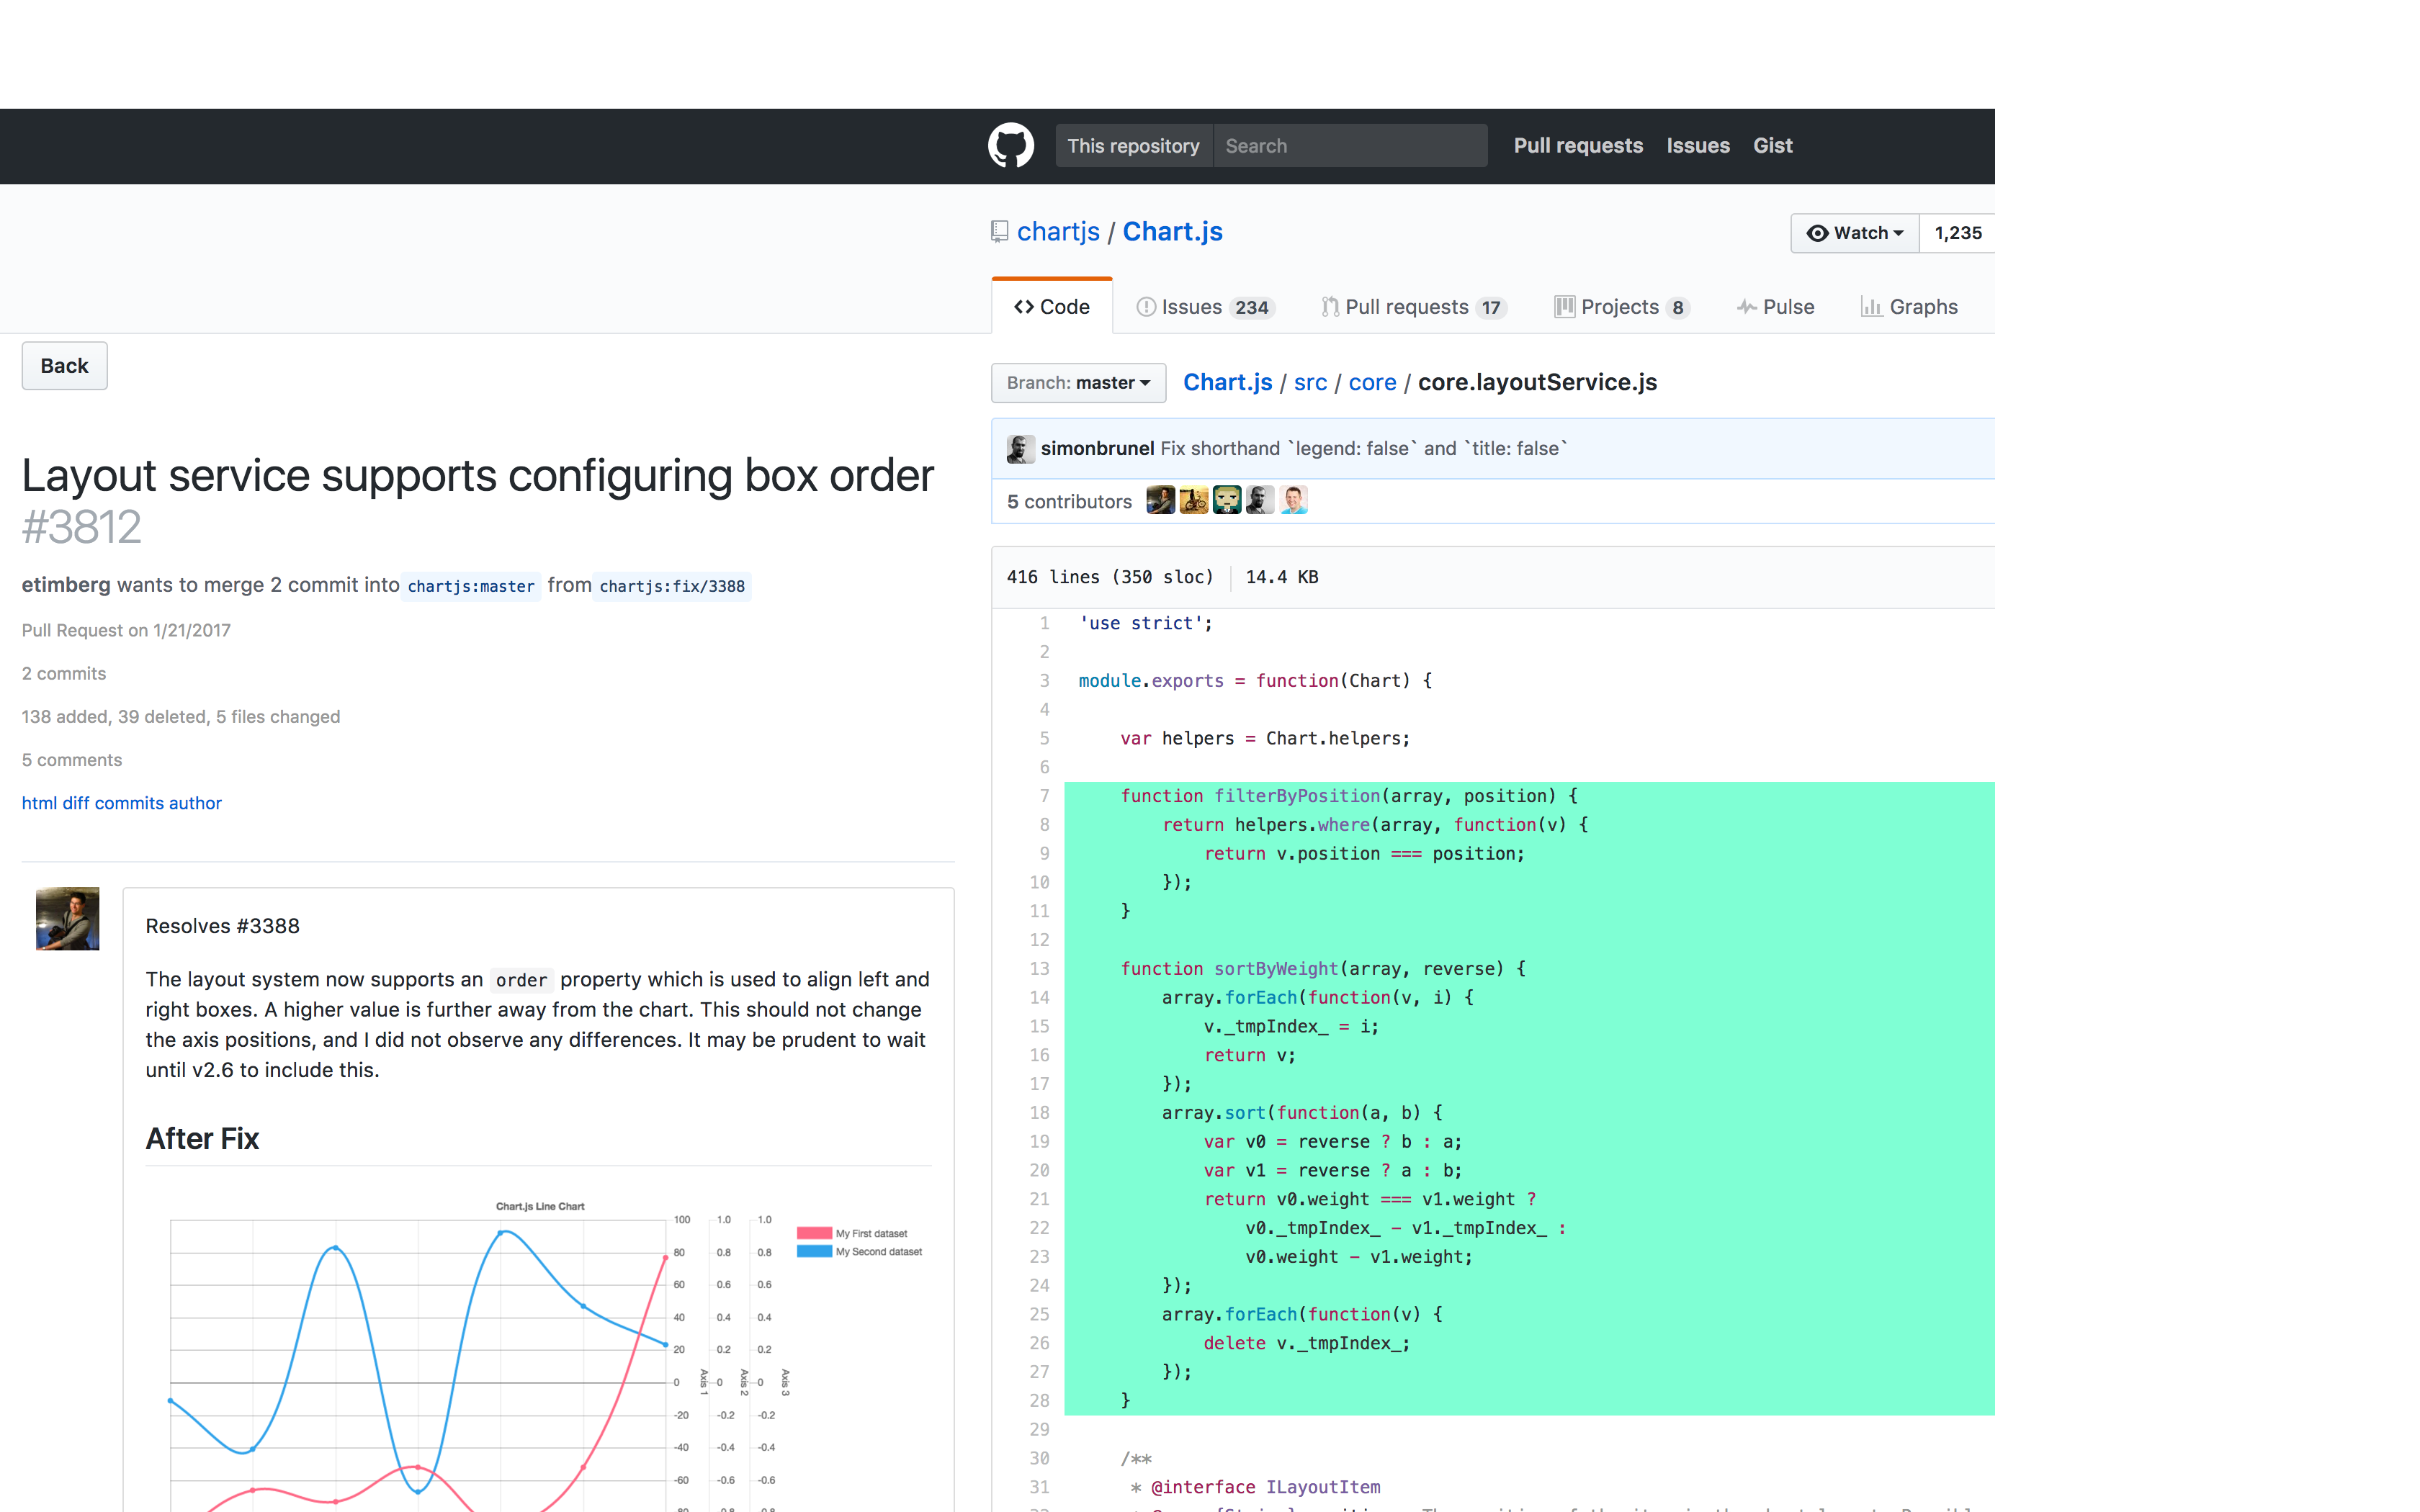
\includegraphics[width=1.2\columnwidth]{interface/top_image.png}
%   \caption{CodeGlass allows users to interactively examine descriptions and comments in pull requests relevant to the chosen portion of code (highlighted in light green). Information in these pull requests can be useful to understand development contexts.}~\label{fig:top}
%   \vspace{-8mm}
% \end{figure}

最近のソフトウェアプロジェクトでは、共同開発や分散開発をサポートするWebサービスであるGitHubが一般的に使用されています。
GitHubはプルリクエストを使ってソフトウェア開発を奨励しています。
プル要求は、コードの変更を説明と共に送信する方法です。
GitHubには、プルリクエストによるレビュープロセスを管理する機能もあります。
多くのプロジェクトではプル要求が積極的に使用されており、開発者はしばしばコード変更に関する詳細情報をそれらに含めます。
我々の形成研究は、プル要求がコード理解を容易にする有益な情報リソースとして役立つ可能性があることを見出した。
この見解は、コード片の理解をサポートするためのインタフェースをどのように設計できるかを検討する動機となる。

このホワイトペーパーでは、CodeGlassと呼ばれるインタラクティブなピースレベルのコード検査ツールを紹介します。
システムは、プルリクエストを抽出し、選択されたコードピースに関連するコメントをレビューする。
このようなやりとりを可能にするために、私たちのピースレベルの差分バックトラックアルゴリズムは、選択したコードピースに関連する過去のコミットとプルリクエストを識別します。
私たちの調査によると、CodeGlassは実装の根拠と開発履歴に関する情報を得るために参加者をサポートできることが明らかになりました。
この作品はヒューマン・コンピュータインタラクションとソフトウェア工学の分野に次の貢献をしています:

\begin{itemize}
\setlength{\parskip}{1mm}
\setlength{\itemsep}{0mm}
	\item 開発者が選択されたコードピースに関連付けられた過去のプルリクエストで説明を表示し、コメントを確認できるように、ピースレベルのコード検査をサポートするためのインターフェイス。
	\item ピースレベルの差分バックトラックアルゴリズムで、指定されたコード片の変更を含む一連のコミットを識別します。
	\item 定量的アルゴリズム評価は、我々のアルゴリズムがコード片の変化を高い精度で取り戻し、想起させることができることを示している。
    \item CodeGlassによるコードの理解と、プロフェッショナルな開発コンテキストでの潜在的なユースケースの改善されたパフォーマンスを明らかにするユーザー評価。
\end{itemize}
